%--- Select slide document and theme ---%
\documentclass{beamer}
\usetheme{Madrid}

%--- Swedish support ---%
\usepackage{fontspec}
\usepackage[swedish]{babel}
%\setmainfont{Palatino Linotype}

%--- verbatim support ---%
\usepackage{verbatim}
\newenvironment{VerbExample}
{\example\semiverbatim}
{\endsemiverbatim\endexample}


%--- Graphics ---%
\usepackage{graphicx}

%--- Label itemize blocks ---%
\usepackage{enumitem}


\begin{document}
\title{FRTN01 project - Group 20}
\subtitle{Control of Batch Tank using Raspberry Pi}
\author{Johan Anderholm \\ Jonathan Kämpe \\ Mikael Sahlström \\ Mikael Nilsson}
\institute[LTH]{LTH}
%\date{\today}

%--- the titlepage frame -------------------------%
\begin{frame}[plain]
  \titlepage
\end{frame}

%--- Slide 1 ---%
\begin{frame}{Project description}
\begin{columns}[T]
    \begin{column}{.55\textwidth}
        Process consists of:
        \begin{itemize}
            \item In pump to control the temperature.
            \item Out pump to control the water level.
            \item Heater to simulate the exothermic process.
            \item Cooler (not used).
            \item Mixer to distribute heatchanges evenly.
        \end{itemize}
    \end{column}
    \begin{column}{.45\textwidth}

        \begin{figure}[H]
           \centering
           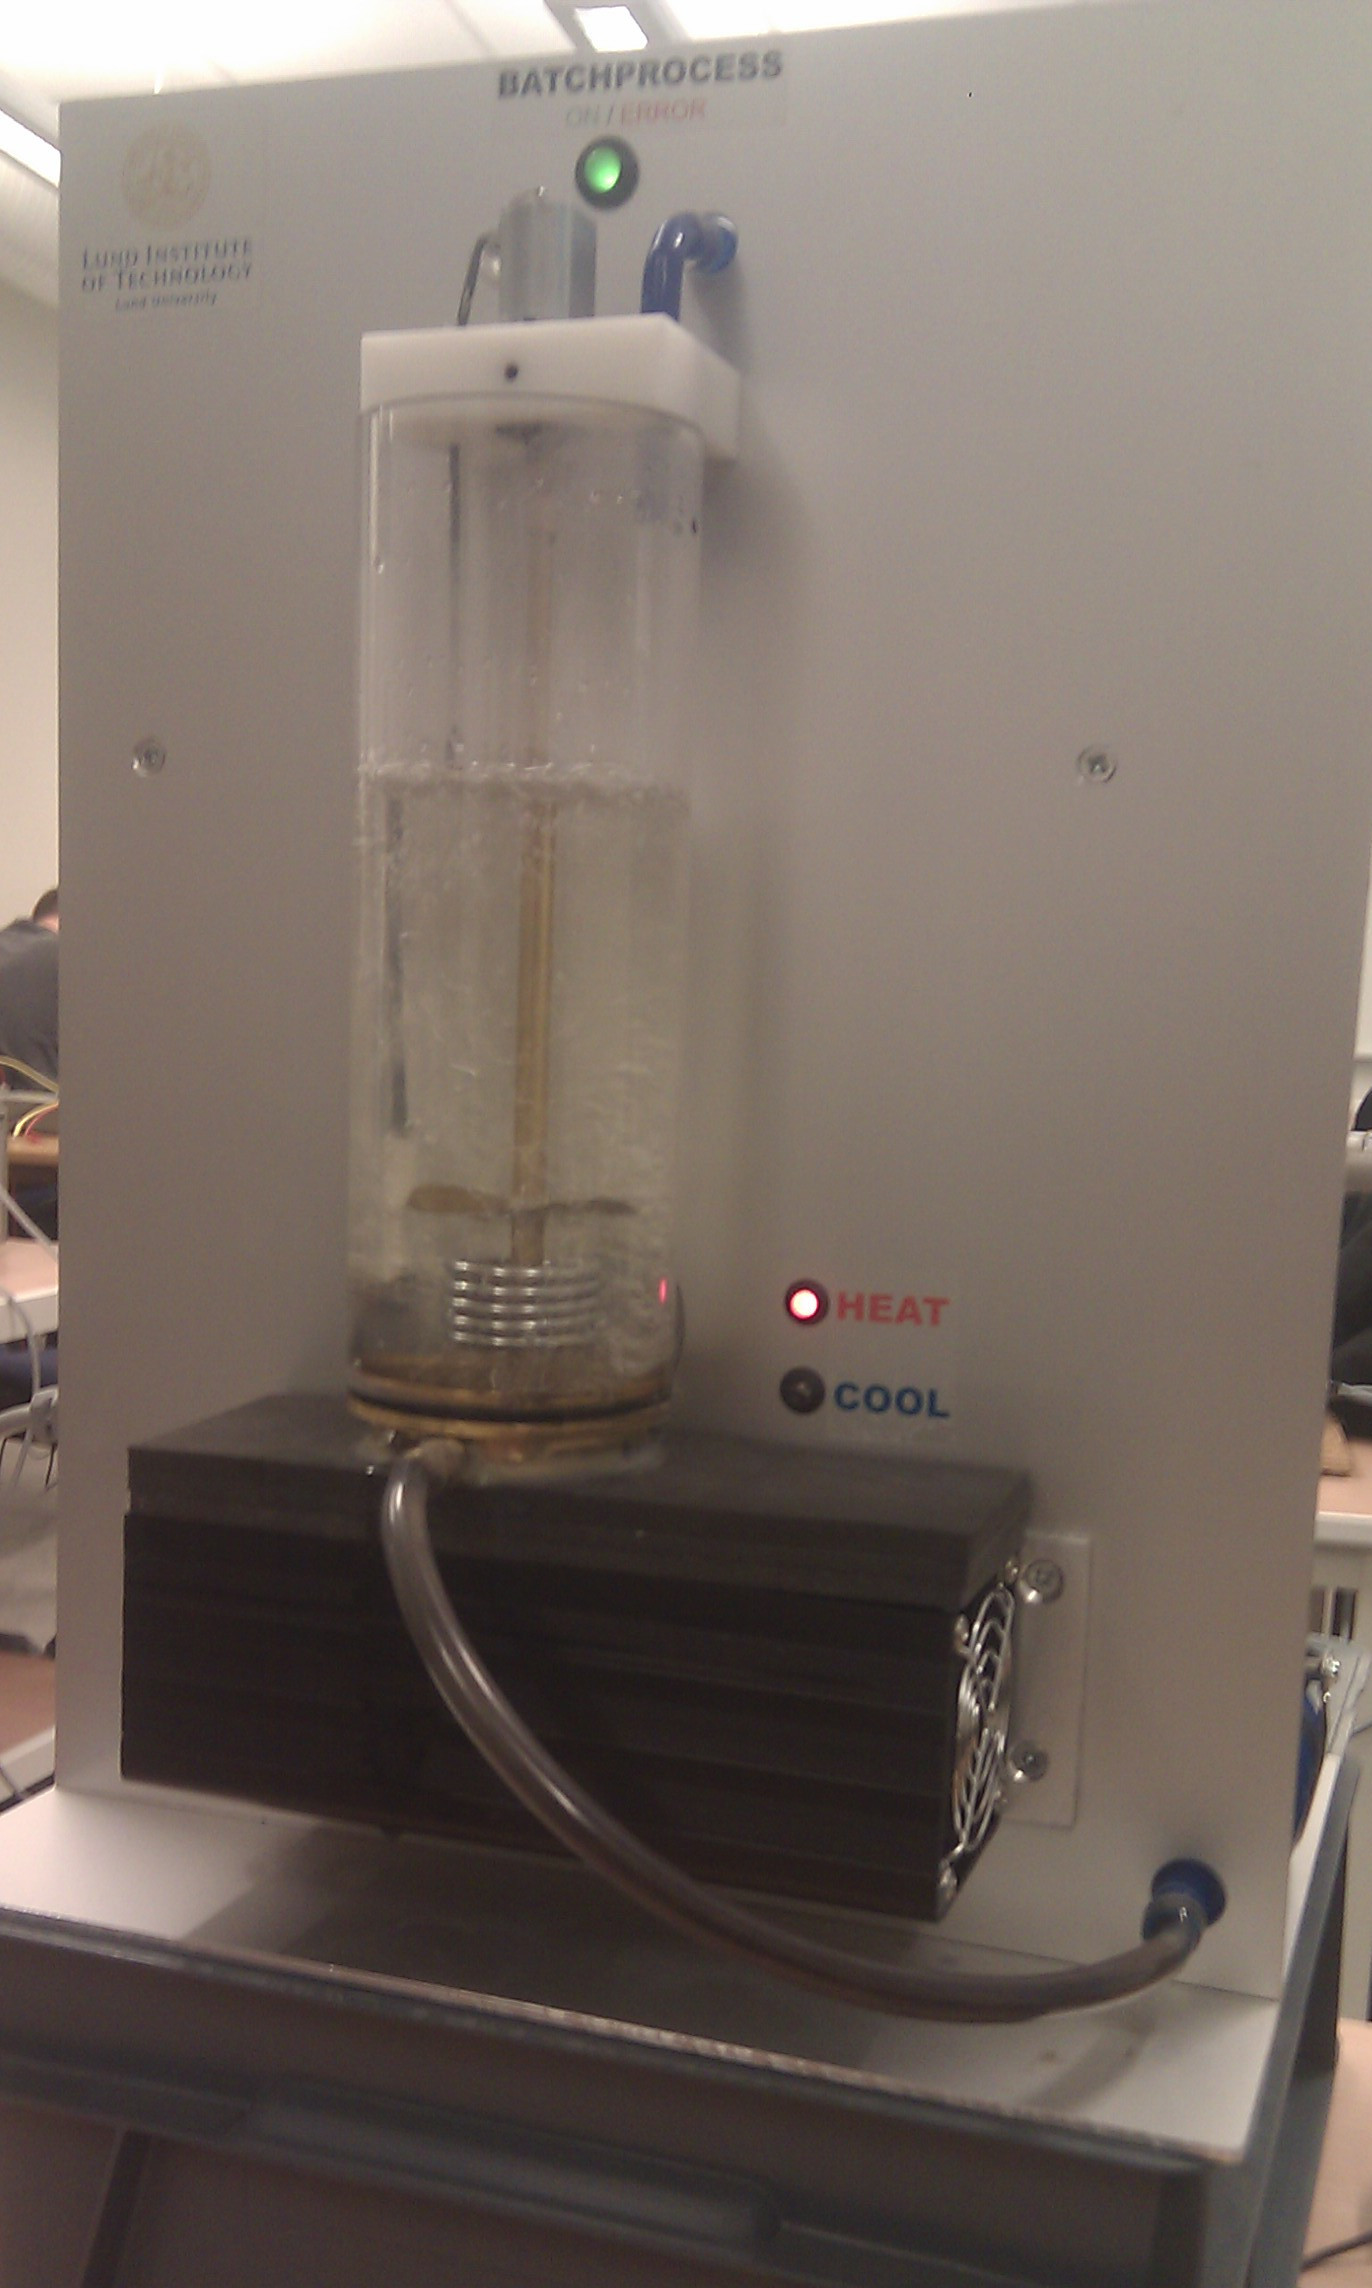
\includegraphics[width=0.7\textwidth]{batchprocess.jpg}
        \end{figure}

    \end{column}
\end{columns}
\end{frame}

%--- Slide 2 ---%
\begin{frame}{System structure}
\begin{columns}[T]
    \begin{column}{.55\textwidth}
        \begin{itemize}
            \item Server/Client that communicates though TCP/IP.
            \item Server is connected to the batchprocess.
            \item Clients receives measurement data from the server and sends control data to the server.
            \item Boost.Threads and Boost.Asio
        \end{itemize}
    \end{column}
    \begin{column}{.45\textwidth}

        \begin{figure}[H]
           \centering
           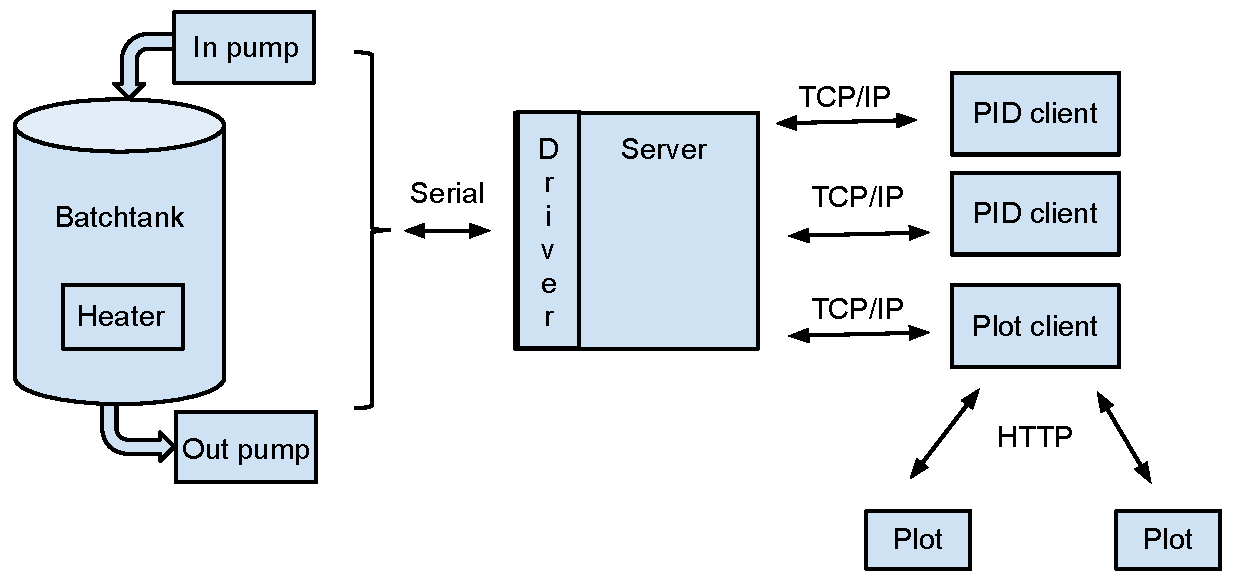
\includegraphics[width=1\textwidth]{systemoverview.pdf}
        \end{figure}

    \end{column}
\end{columns}
\end{frame}

%--- Slide 2 ---%
\begin{frame}{Server}
\begin{columns}[T]
    \begin{column}{.55\textwidth}
        \begin{itemize}
            \item Communicates with the batchprocess over a serial interface though a driver.
            \item Listens for connections from clients.
            \item Takes measurement data from the batchprocess and sends to the clients upon their request.
            \item Receives control data from the clients and send it to the batchprocess.
        \end{itemize}
    \end{column}
    \begin{column}{.45\textwidth}

        \begin{figure}[H]
           \centering
         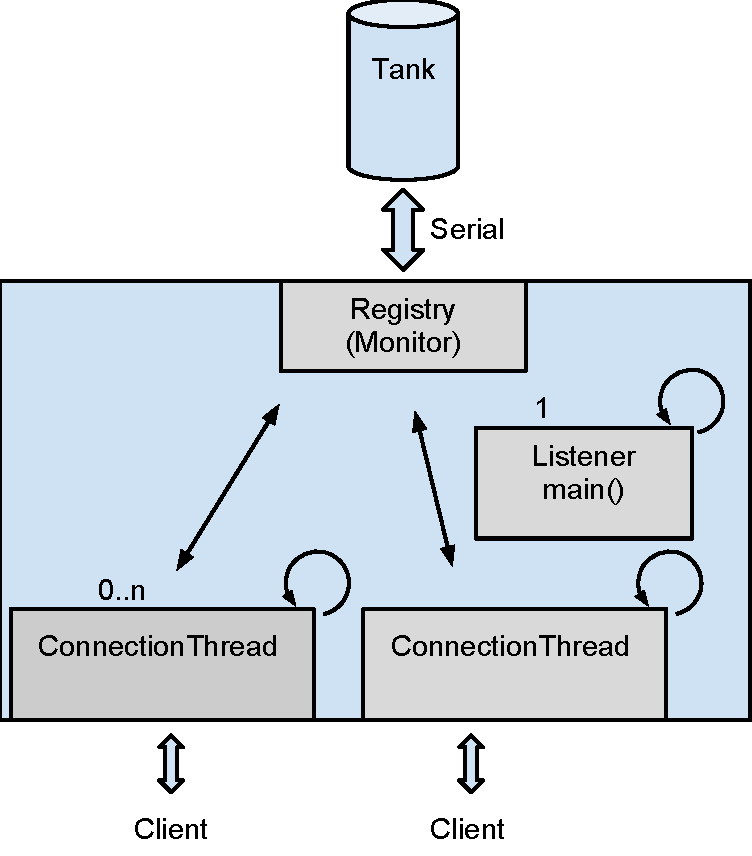
\includegraphics[width=1\textwidth]{server_sketch.pdf}
        \end{figure}

    \end{column}
\end{columns}
\end{frame}

\begin{frame}[fragile]
\frametitle{Protocol Buffers}
\begin{columns}
    \begin{column}{.5\textwidth}
    \normalsize
    Message definition.
    \footnotesize
    \begin{verbatim}
message Register {
  required uint64 period = 1;
}

message Sample {
  required int32 value = 1;
}

message BaseMessage {
  optional Sample sample = 1;
  optional Register register = 2;
}
\end{verbatim}
    \end{column}
    \begin{column}{.4\textwidth}
    \normalsize
    Compiled code.
    \footnotesize
    \begin{verbatim}
MessageInput in(*m_Socket);
BaseMessage msg;

// Read message
in >> msg;

if (msg.hasregister()) {
   Register* r = msg.register()
   uint64_t period = r.period();
   // Do stuff.
}
\end{verbatim}
    \end{column}
\end{columns}
\end{frame}


%--- Slide 3 ---%
\begin{frame}{Driver}
        \begin{itemize}
            \item Driver for communicating with the batchprocess over a serial interface.
            \item Uses the Unix API termios.
            \item Uses standard C functions for I/O; read(2), write(3), open(2), close(2).
            \item Sends and receives data in chunks of 8 bits, the data is raw.
            \item Time out after 1 sec of no response.
        \end{itemize}
\end{frame}

%--- Slide 4 ---%
\begin{frame}[fragile]
    \frametitle{Protocol - as seen in the source code of the batch tank}
        \small
\begin{semiverbatim}
+-+-+-+-+-+-+-+-+
|0|cmd|  chan   | 
+-+-+-+-+-+-+-+-+

00 = bit clear, 01 = bit set, 10 = bit get, 11 = chan get

+-+-+-+-+-+-+-+-+  +-+-+-+-+-+-+-+-+ 
|1| bit8...bit2 |  |0|bit|  chan   |
+-+-+-+-+-+-+-+-+  +-+-+-+-+-+-+-+-+ 

+-+-+-+-+-+-+-+-+  +-+-+-+-+-+-+-+-+  +-+-+-+-+-+-+-+-+ 
|1|bit15...bit9 |  |1| bit8...bit2 |  |0|bit|  chan   |
+-+-+-+-+-+-+-+-+  +-+-+-+-+-+-+-+-+  +-+-+-+-+-+-+-+-+ 
 
+-+-+-+-+-+-+-+-+  +-+-+-+-+-+-+-+-+     +-+-+-+-+-+-+-+-+ 
|1|bit31...bit30|  |1|bit29...bit23| ... |0|bit|  chan   |
+-+-+-+-+-+-+-+-+  +-+-+-+-+-+-+-+-+     +-+-+-+-+-+-+-+-+ 
\end{semiverbatim}
\end{frame}


%--- Slide 5 ---%
\begin{frame}{Clients}
	\begin{itemize}
   		\item Plotting, PID, Manual control.
        \item Connects to server.
		\item Communicates with protobuf messages.
    \end{itemize}
\end{frame}

%--- Slide 6 ---%
\begin{frame}{Plot client}
	\begin{itemize}
    	\item A client that is an HTTP server.
        \item Receives measurement data and control data from the server.
        \item Listens for HTTP connections on port 8080.
        \item Serves a HTML, CSS and Javascript based plotting system.
        \item The plotting system sends AJAX GETs to the HTTP server which answers with the latest data.
        \item Plots multiple curves on multiple plots.
    \end{itemize}
\end{frame}

%--- Slide 7 ---%
\begin{frame}{PID clients}
	\begin{itemize}
		\item C++, boost:asio.
		\item Parameters in .ini files updates on the go.
		\item Registers for periodic sampling.
		\item Responds on each sample with a new control signal.
		\item FAI, BAD, bumpless transfer, tracking.
		\item Parameters chosen by empirical studies.
	\end{itemize}
\end{frame}

%--- Slide 8 ---%
\begin{frame}{PID.ini}
\begin{columns}[T]
	\begin{column}{.5\textwidth}
%		\begin{verbatim}
[General]\\
ipaddress = 130.235.83.235\\
port = 54000\\
sensor = TEMP\\
output = IN PUMP\\
period = 50\\
delay = 0\\
%		\end{verbatim}
	\end{column}

	\begin{column}{.5\textwidth}
%		\begin{verbatim}
[PID]\\
K = 10\\
Ti = 10\\
Td = 0\\
Tr = 1\\
N = 0\\
ref = 370\\
umin = 0\\
umax = 200\\
inverted = true\\
%		\end{verbatim}
	\end{column}
\end{columns}
\end{frame}

%--- Slide 9 ---%
\begin{frame}{PID client}
	\begin{figure}
		\center
		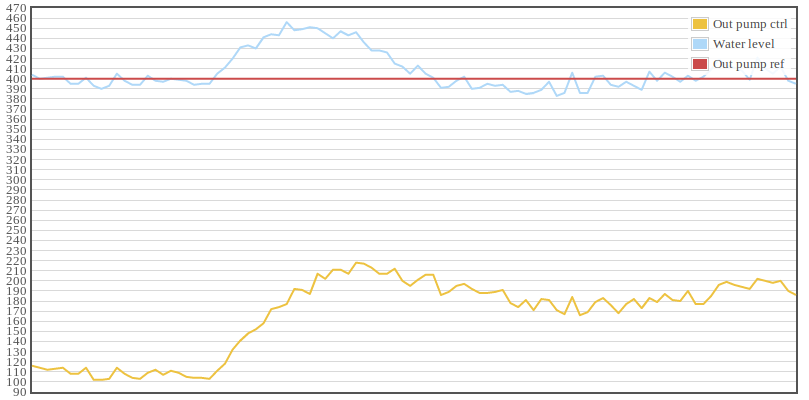
\includegraphics[width=0.8\textwidth]{plot1.png}
	\end{figure}
	\begin{itemize}
		\item PID client controlling the out pump based on water level reference value set to 400 while manually controlling in pump to create a response.
		\item High frequency noise due to the water stream from the in pump. Will not affect out pump power that much due to inability to change pumping power fast.
    \end{itemize}
\end{frame}
\end{document}
